{
\abnormalparskip{0pt}
\chapter{Experiments}
\label{cha:experiments}
}

This chapter describes and discuss the experiments that has been performed in
relation to the new implementation.

All experiments has been executed on computer with $8 \times$ Intel\textsuperscript{\textregistered}
Xeon\textsuperscript{\textregistered} CPU E5-2630L at $2.00$ GHz and with $16$ GB
RAM. Furthermore all tests was executed using version $1.4.2$ of Go\footnote{A newer 1.5
which ups the performance of the language due to more efficient garbage
collection was released after the experiments had been conducted.}.
%
\begin{table}[htbp]
  \centering
  \begin{tabular}{cp{9cm}}
    \toprule
    Method       & Description                                      \\
    \midrule
    \texttt{Simple}       & New implementation with the analytical method.   \\
    \texttt{SimpleSort}   & New implementation with the analytical method and sorted
                   terminals.                                       \\
    \texttt{SmithNew}     & New implementation with \citeauthor{smith1992}'s
                   iteration.                                       \\
    \texttt{SmithNewSort} & New implementation with \citeauthor{smith1992}'s iteration
                   and sorted terminals.                            \\
    \texttt{SmithOld}     & Original implementation by \textcite{smith1992}. \\
    \bottomrule
  \end{tabular}
  \caption[Naming of methods]{The naming of methods has been done in the
    experiments as shown here.\label{tab:method-names}}
\end{table}
%
In the experiments the used methods are named as seen in
\cref{tab:method-names}.

In general the type of experiments which has been performed, relates to either
correctness or performance of the implementation. The correctness has been
measured by comparing a set of instances with the results found by the
GeoSteiner program. The performance experiments is divided into experiments
regarding the speed of the methods, the number of trees which are optimized, and
the number of iterations being run. 

\section{Correctness}
\label{sec:correctness}

To test the correctness of the new implementation $150$ random cube instances
with $n = 10 \ldots 12$ and $d = 2$ has been run. The cube instances are the
same used by \textcite{fonseca2014}, which can also be found in
\url{https://github.com/DIKU-Steiner/MPC15/tree/master/experiments/Correctness/Instances}. The
experiments was run for the two methods of the new implementation, both with and
without sorting of terminals. To compare with, the instances was also run using
the official GeoSteiner implementation, which can be found at
\url{http://geosteiner.com}.

After all instances was run, the results of the new implementation was compared
with the results of the GeoSteiner program. This showed, that simple method,
both with and without sorting, in a few instances gave sub-optimal
\acp{mst}. These and the difference to the optimal \ac{mst} found by GeoSteiner
can be found in \cref{tab:correctness-errors}.
%
\begin{table}[htbp]
  \centering
  \begin{tabular}{ccc}
    \toprule
    Instance           & Method              & Diff       \\
    \midrule
    cube\_n12\_d2\_s27 & \texttt{Simple}     & $+0.170\%$ \\
    cube\_n12\_d2\_s49 & \texttt{Simple}     & $+0.295\%$ \\
    cube\_n10\_d2\_s42 & \texttt{SimpleSort} & $+0.015\%$ \\
    cube\_n12\_d2\_s26 & \texttt{SimpleSort} & $+0.228\%$ \\
    cube\_n12\_d2\_s43 & \texttt{SimpleSort} & $+0.292\%$ \\
    cube\_n12\_d2\_s49 & \texttt{SimpleSort} & $+0.295\%$ \\
    \bottomrule
  \end{tabular}
  \caption[Suboptimal \acsp{mst} in correctness test]{The table shows the
    instances in which some method gave sub-optimal results, and the difference
    in percent to the optimal \acp{mst} found by the GeoSteiner
    program.\label{tab:correctness-errors}}
\end{table}
%
As can be seen \texttt{Simple} gave sub-optimal results in $2$ instances, and
\texttt{SimpleSort} in in $4$ instances, meaning that $6$ of $300$ ($2\%$) instances
gave sub-optimal results, or.

When inspecting the \acp{mst} generated by the simple method in the sub-optimal
instances, it was clear, that the method in these case indeed gave \acp{mst}
which were slightly different from the \ac{smt} found by either GeoSteiner or
with \citeauthor{smith1992}'s iteration. 

The reason for this seems to lie with to things, one the condition of the main
loop which decides is we skip a topology, and two the error function.

Firstly, in the original implementation in the main loop, \textit{before} any
optimization has taken place, the length and error of the tree is calculated. A
check is then performed to see whether the length minus the error is greater
than the upper bound, and if so the topology vector and all its descendants are
skipped. If this is not the case, the tree is optimized once if its error is
greater than the length times $0.005$. It then loops back and once again
calculates the length and error. There are two ways out of this loop. Either the
first if-clause fails, and we discard the topology vector and its descendants,
or the tree is optimized enough that the code second if-clause is false and we
continue on with the code (as there is only that first single \texttt{goto}).
The relevant code snippet can be found in~\cref{fig:loop-condition-pruning}. 
%
\begin{figure}[htbp]
\begin{c-code}
  ITER: /* .. and optimize it until either obviously bad
              or small error figure happens */
    q = length();
    r = error();
    if ( q - r < STUB) {
      if (r > 0.005*q) { optimize(0.0001*r/NUMSITES); goto ITER; }
      // ... Truncated code
    }
\end{c-code}
  \captionof{listing}[Loop condition for pruning topologies]{The outer if-clause
    decides whether we prune a topology or not. This is applied before the
    topology is optimized to its \acs{rmt}, which significantly speeds up the
    program. But whether this is allowed is unclear.\label{fig:loop-condition-pruning}}
\end{figure}
%
The new implementation has retained this structure in the main loop, as it
significantly speeds up the program. However, as described earlier, there is no
clear link between the error and the length of the tree. Thus the outer
if-clause is indeed a bit sketchy as \texttt{STUB} is the length of a fully
optimized tree, whereas $q - r$ is the length of a possibly still yet to be optimized
tree minus its error. Thus this assumes that one can subtract the error, and
always get a length which is the same or smaller than the length of the fully
optimized tree. If this is not the case, we may actually discard a topology
vector which could lead to the \ac{mst}.

However this does indeed seem to go right when using the iteration proposed by
\textcite{smith1992} and therefore one may ask the question why it sometimes
fails for the method using the analytical solution.

The reason for this, I believe, is two-fold: Firstly when optimizing using the
analytical solution one in general gets an error which is much smaller than the
one found when using \citeauthor{smith1992}'s iteration. This is due to the fact
that we place the Steiner points at their exact position when optimizing them.
Because the error becomes so much smaller, we could imagine a situation in which
we have optimized a tree with e.g.\ $4$ terminals. When we then insert the $5$th
terminal because the error of the rest of the tree is so small we will not
optimize the tree when we reach the second if-clause---even if the $5$th point
is at a sub-optimal placement. Secondly, if the first if-clause is faulty, then
it may go well with \citeauthor{smith1992}'s iteration because the error of all
Steiner points tend to follow each other, and also in general only goes slightly
below the optimization stop-criteria. However when using the analytical solution
the error becomes so much smaller, that we may risk discarding a topology vector
for which we could have a optimized, e.g.\ the Steiner point from when we
inserted the before described $5$th terminal, to get the length below the upper
bound. These two factors together, I believe to be the source of the bug.

I believe this bug could be fixed firstly by not using the error of the entire
tree, but instead look at the error of each Steiner point (similar to
the way the simple method is presented in \cref{sec:simple-iteration}). Thus we
only stop optimizing (the inner if-clause) when the error of all Steiner points,
considered independently, falls below some threshold. Secondly, it is possible
that one has to wait with the check as to whether we can prune a topology vector
until we have optimized it to its respective \ac{rmt}. Both of these
modifications, especially the second, are at the risk of increasing the number
of iterations, trees and thus run-time of the program.

The bug as it is described here has not been fixed at this point, due to the
lack of time, and all of the below tests has been performed using this
implementation. As such this is something we have to keep in mind when comparing
the performance of the implementations and methods. However I do not believe it
invalidates the data, as the number of sub-optimal trees in the correctness test,
was still very low, and the sub-optimality of these trees also was relatively
low.

\section{Performance}
\label{sec:performance}

To test the performance of the implementation the test sets in
\cref{tab:test-sets} has been run for all of the methods described in
\cref{tab:method-names}. All sets have been taken from \textcite{fonseca2014},
but the sets Carioca and Cube has been pruned. This has been done due to the
sheer size of these sets. Even with these sets pruned, running all of the sets
for all of the methods took a little more than a week in which a quad-core
computer ran 24/7. To further prune, all runs was set up such that they would
halt if more than $12$ hours passed, as it is then concluded infeasible to solve
that specific instance using the given method. How many instances completed
before the time limit can be seen in~\cref{tab:set-success}.

A few initial test runs showed that, especially \texttt{SimpleSort} but also
occasionally \texttt{SmithNewSort}, were able to solve several instances with
$n=16$, and a few for $n=17$ within the $12$ time limit. Time-wise it was
however still infeasible to perform a proper test with these instance sizes.
Thus the new implementation solves instances about the same size as
\textcite{fonseca2014}.
%
\begin{table}[htbp]
  \centering
  \begin{tabular}{ccccc}
    \toprule
    Set     & Dimensions       & Terminals             & Set size & Point configuration \\
    \midrule
    Carioca & $d = 3 \ldots 5$ & $n = 11 \ldots 16$    & $90$     & Random in cube      \\
    Cube    & $d = 2 \ldots 4$ & $n = 10 \ldots 15$    & $360$    & Random in cube      \\
    Iowa05  & $d = 3 \ldots 5$ & $n = 10$              & $30$     & Random in cube      \\
    Sausage & $d = 2 \ldots 5$ & $n = 10 \ldots 15$    & $24$     & Simplex sequence    \\
    Solids  & $d = 3$          & $n = 4, 6, 8, 12, 20$ & $5$      & Platonic solids     \\
    \bottomrule
  \end{tabular}
  \caption[Test sets used to test performance]{The table shows the tests sets,
    their dimensions, number of terminals, number of instances and type of instances,
    which has been used to test the performance of the implementation.\label{tab:test-sets}}
\end{table}
%
\NOTE[inline]{Currently it appears that I do not use Iowa05 and Solids for anything.
  Possibly I should also use this?}
%
The data collected from the runs have been used to compare the speed (i.e.\
run-time), the number of iterations, and the number of trees optimized. The
results are presented and described in the two sections below.
%
\begin{table}[htbp]
  \centering
  \begin{tabular}{cccccc}
    \toprule
            & \multicolumn{5}{c}{Method}                               \\
    \cmidrule(l){2-6}
    Set     & \texttt{Simple} 
            & \texttt{SimpleSort}
            & \texttt{SmithNew} 
            & \texttt{SmithNewSort}
            & \texttt{SmithOld}                                        \\
    \cmidrule(r){1-1}\cmidrule(l){2-6}
    Carioca & $81$   & $89$       & $73$     & $87$         & $76$     \\
    Cube    & $360$  & $360$      & $352$    & $360$        & $356$    \\
    Iowa05  & $30$   & $30$       & $30$     & $30$         & $30$     \\
    Sausage & $22$   & $23$       & $18$     & $22$         & $21$     \\
    Solids  & $4$    & $4$        & $4$      & $4$          & $4$      \\
    \bottomrule
  \end{tabular}
  \caption[Successfull test runs]{The table shows the number of successfull
    instances, i.e.\ instances which finished within $12$ hours, of the test
    sets which has been run. The number of instances for each test set can be
    seen in~\cref{tab:test-sets}.\label{tab:set-success}}
\end{table}

\subsection{Speed}
\label{sec:speed}

\begin{figure}[htbp]
  \centering
  \begin{subfigure}[t]{0.5\textwidth}
    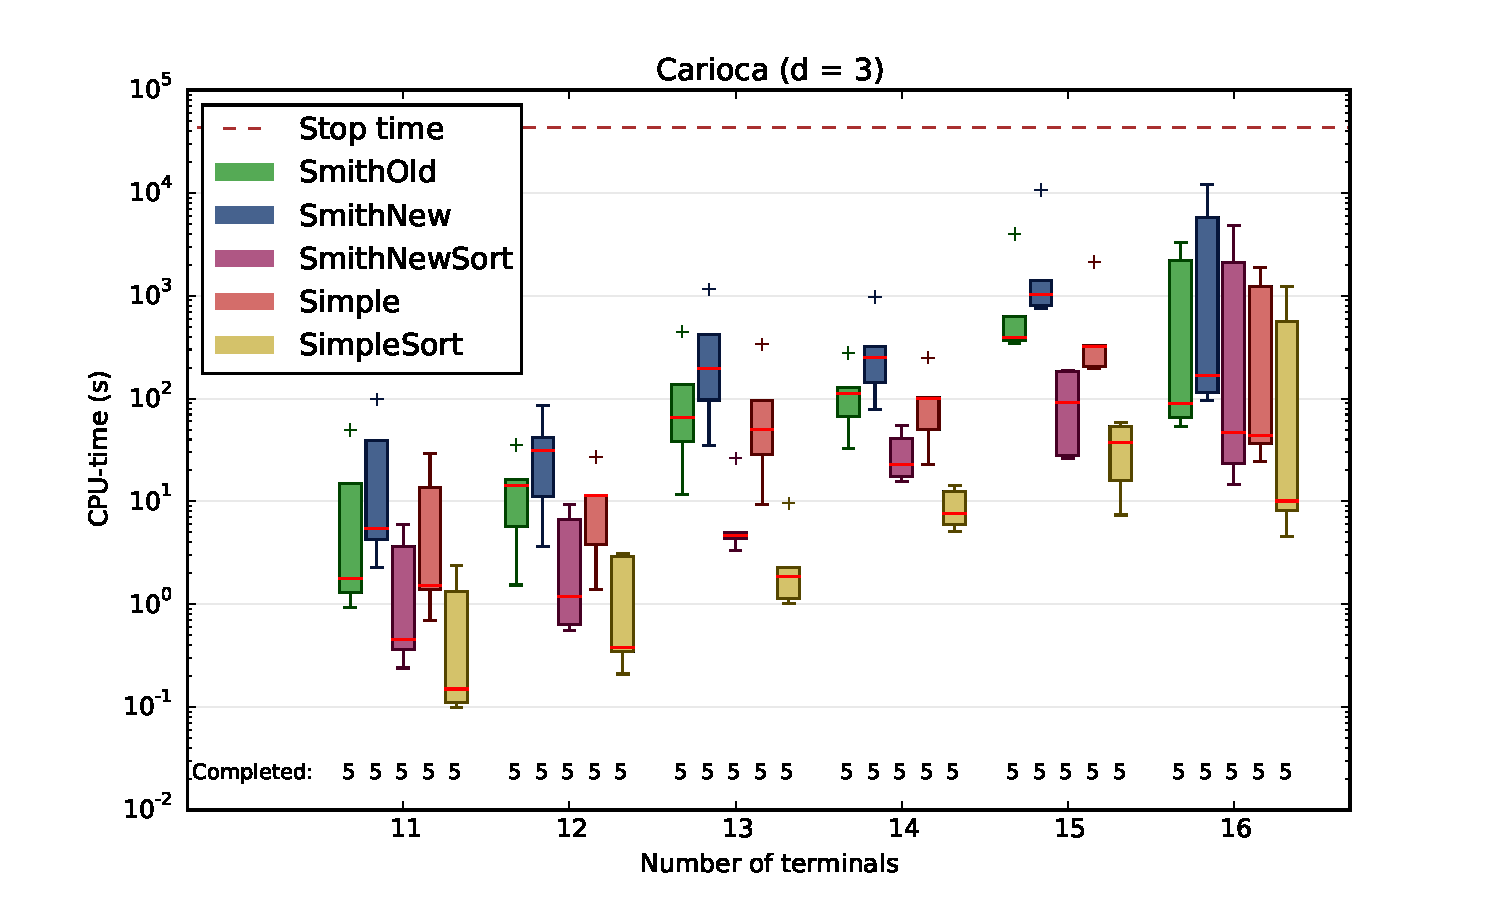
\includegraphics[width=\textwidth]{gfx/boxplots/plot_nvst_boxplot_d3_Carioca_1}
  \end{subfigure}%
  \begin{subfigure}[t]{0.5\textwidth}
    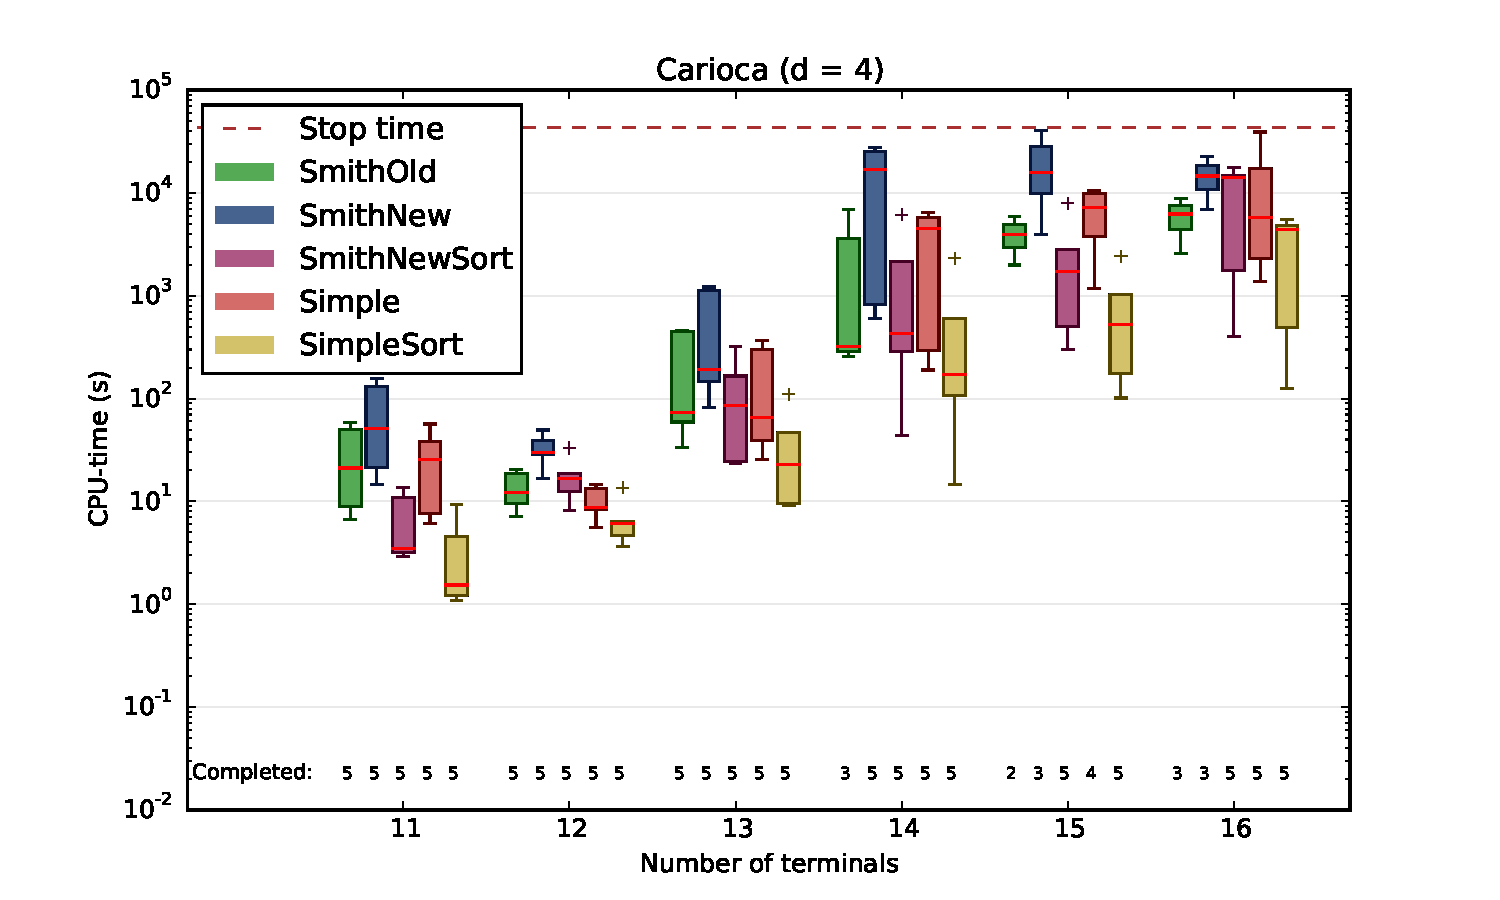
\includegraphics[width=\textwidth]{gfx/boxplots/plot_nvst_boxplot_d4_Carioca_1}
  \end{subfigure}
  \begin{subfigure}[t]{0.5\textwidth}
    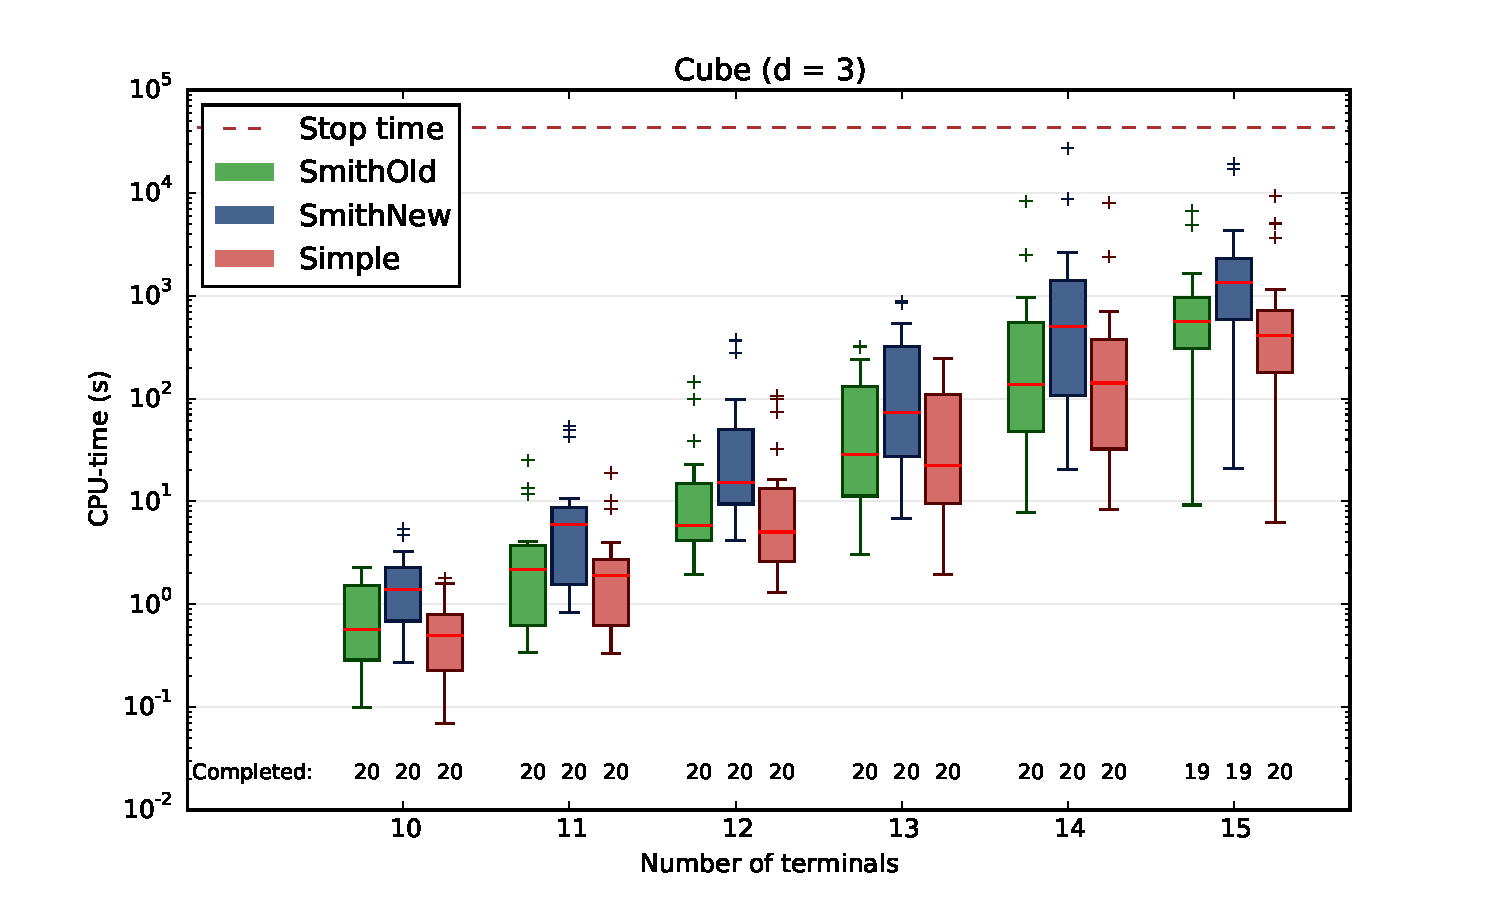
\includegraphics[width=\textwidth]{gfx/boxplots/plot_nvst_boxplot_d3_Cube_1}
  \end{subfigure}%
  \begin{subfigure}[t]{0.5\textwidth}
    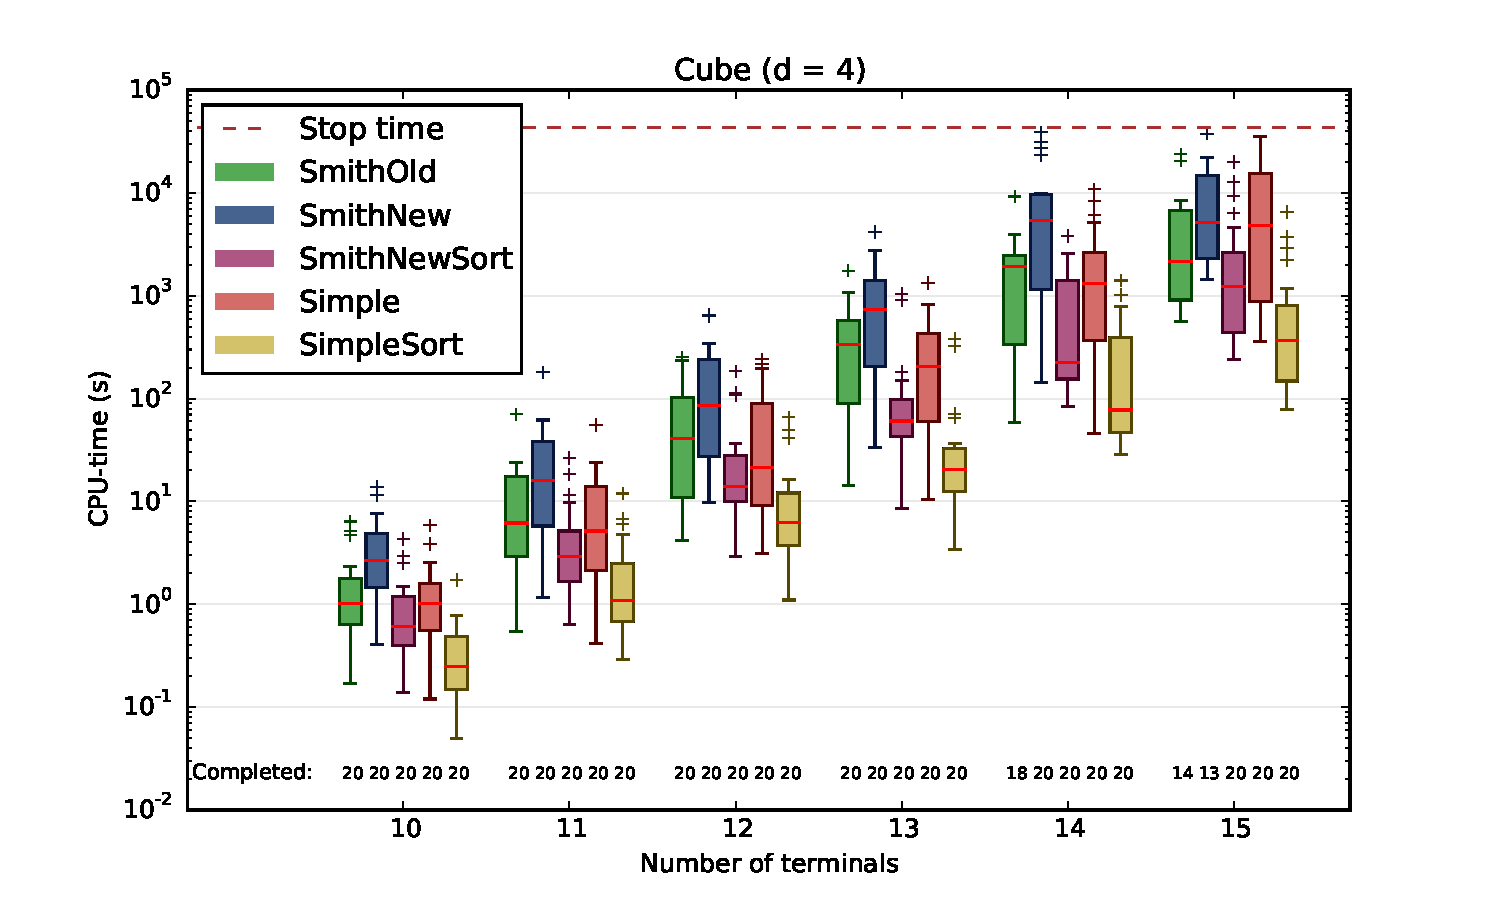
\includegraphics[width=\textwidth]{gfx/boxplots/plot_nvst_boxplot_d4_Cube_1}
  \end{subfigure}%
  \caption[Box-plots: \texttt{SmithOld} vs.\ \texttt{SmithNew} vs.\
  \texttt{Simple}]{Box-plots for the Carioca and Cube set for $d = 3, 4$. The
    plots compare the three methods \texttt{SmithOld}, \texttt{SmithNew} and
    \texttt{Simple}. The red bar is the second quartile (the median), the boxes
    are the first and third quartiles, the whiskers show the lowest datum still
    within $1.5$ IQR of the first and third quartile. Finally every $+$ is a datum
    outside of the whiskers, i.e.\ outliers. The numbers at the bottom shows the
    number of instances which completed (and thus has been used to calculate the
    box-plot) before the stop time of $12$ hours.\label{fig:boxplots-1}}
\end{figure}
%
To compare the speed of the new implementation with the implementation by
\textcite{smith1992} a box-plot of the run times for the Carioca set and Cube
set, where $d = 3$ and $d = 4$, has been plotted in \cref{fig:boxplots-1}. As
can be seen by the two figures the running time of \texttt{SmithNew} is in
general a bit higher than that of \texttt{SmithOld}, whereas the new analytical
solution \texttt{Simple} in general is lower. The reason for the higher running
time of \texttt{SmithNew} is probably due to the fact that the implementation is
done in Go instead of C as the original implementation. Unfortunately we are
therefore not really able to say anything about the performance of the new data
structure for topologies (described in~\cref{sec:building-topologies}) being
better of worse than the original implementation. It is however interesting to
see that the analytical solution seems to have better running times than not
only \texttt{SmithNew}, but also \texttt{SmithOld}, as this suggests that an
implementation of this method in a more efficient language, such as C, would
yield even better running times. Further this seems to debunk the claim by
\textcite{smith1992} that a simple iteration would converge slower, at least
speed-wise. Of course we still need to keep in mind the fact that
\texttt{Simple} have showed some sub-optimal trees. It however seems unlikely,
when looking at the percent of sub-optimal results that this should skew the
results so much that this would be changed.
% 
\begin{figure}[htbp]
  \centering
  \begin{subfigure}[t]{0.5\textwidth}
    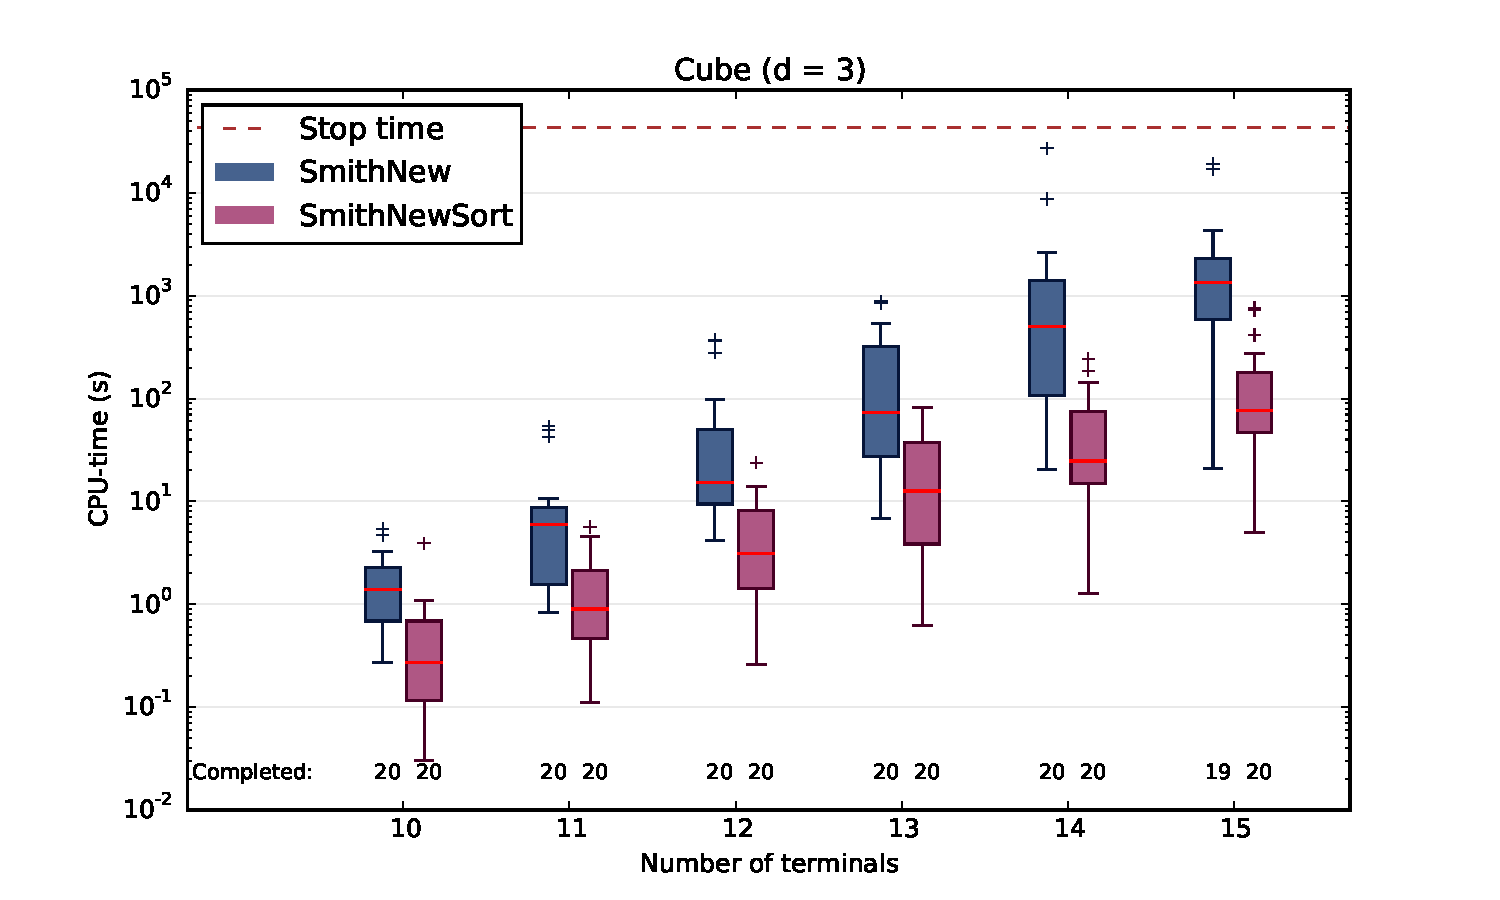
\includegraphics[width=\textwidth]{gfx/boxplots/plot_nvst_boxplot_d3_Cube_2}
  \end{subfigure}%
  \begin{subfigure}[t]{0.5\textwidth}
    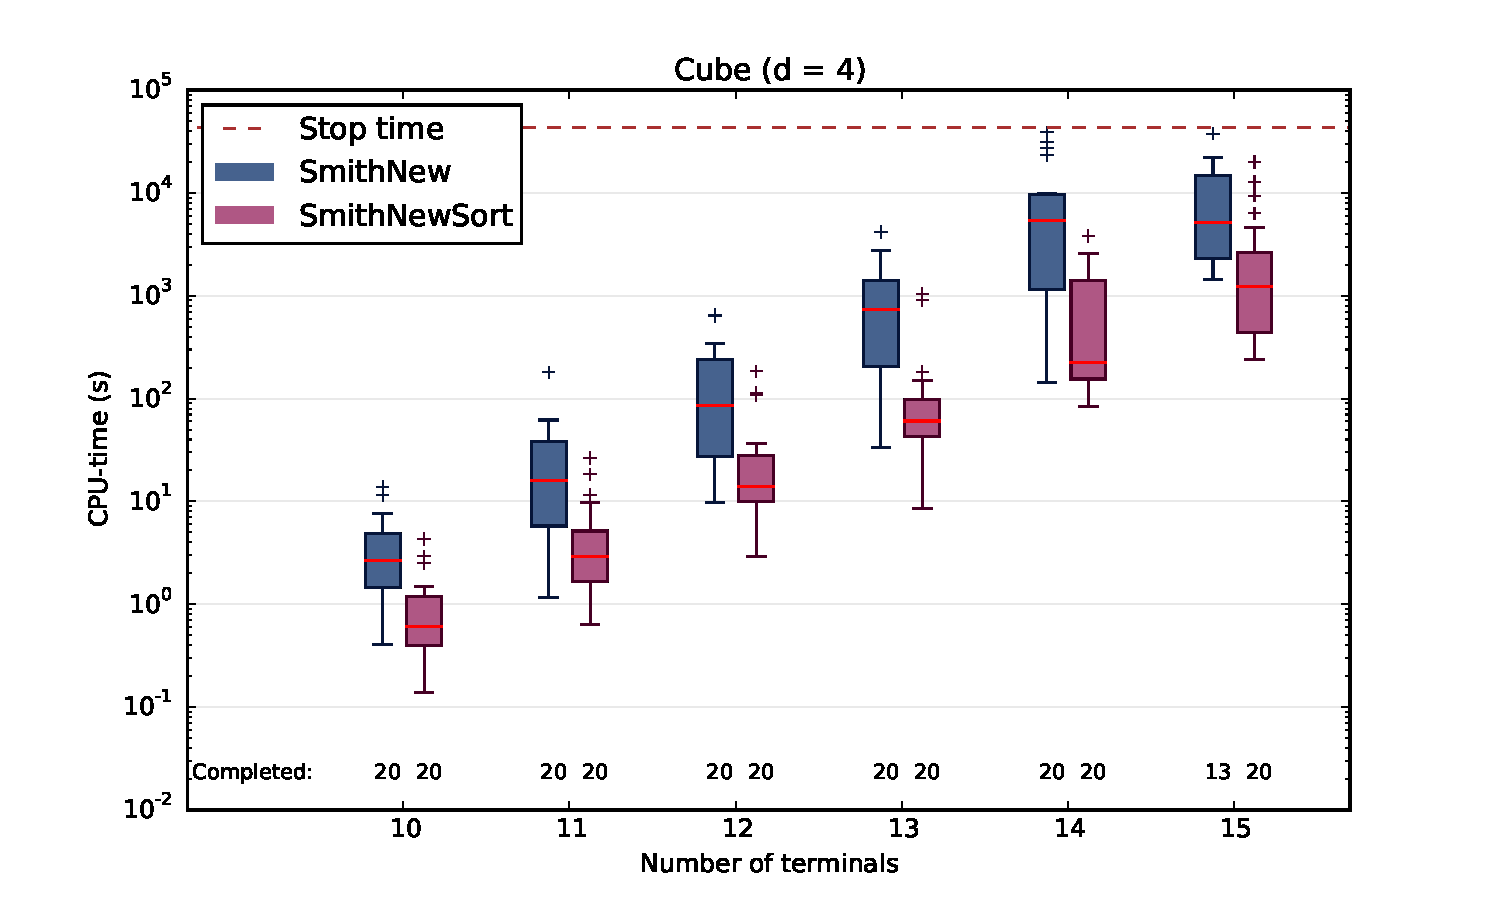
\includegraphics[width=\textwidth]{gfx/boxplots/plot_nvst_boxplot_d4_Cube_2}
  \end{subfigure}
  \begin{subfigure}[t]{0.5\textwidth}
    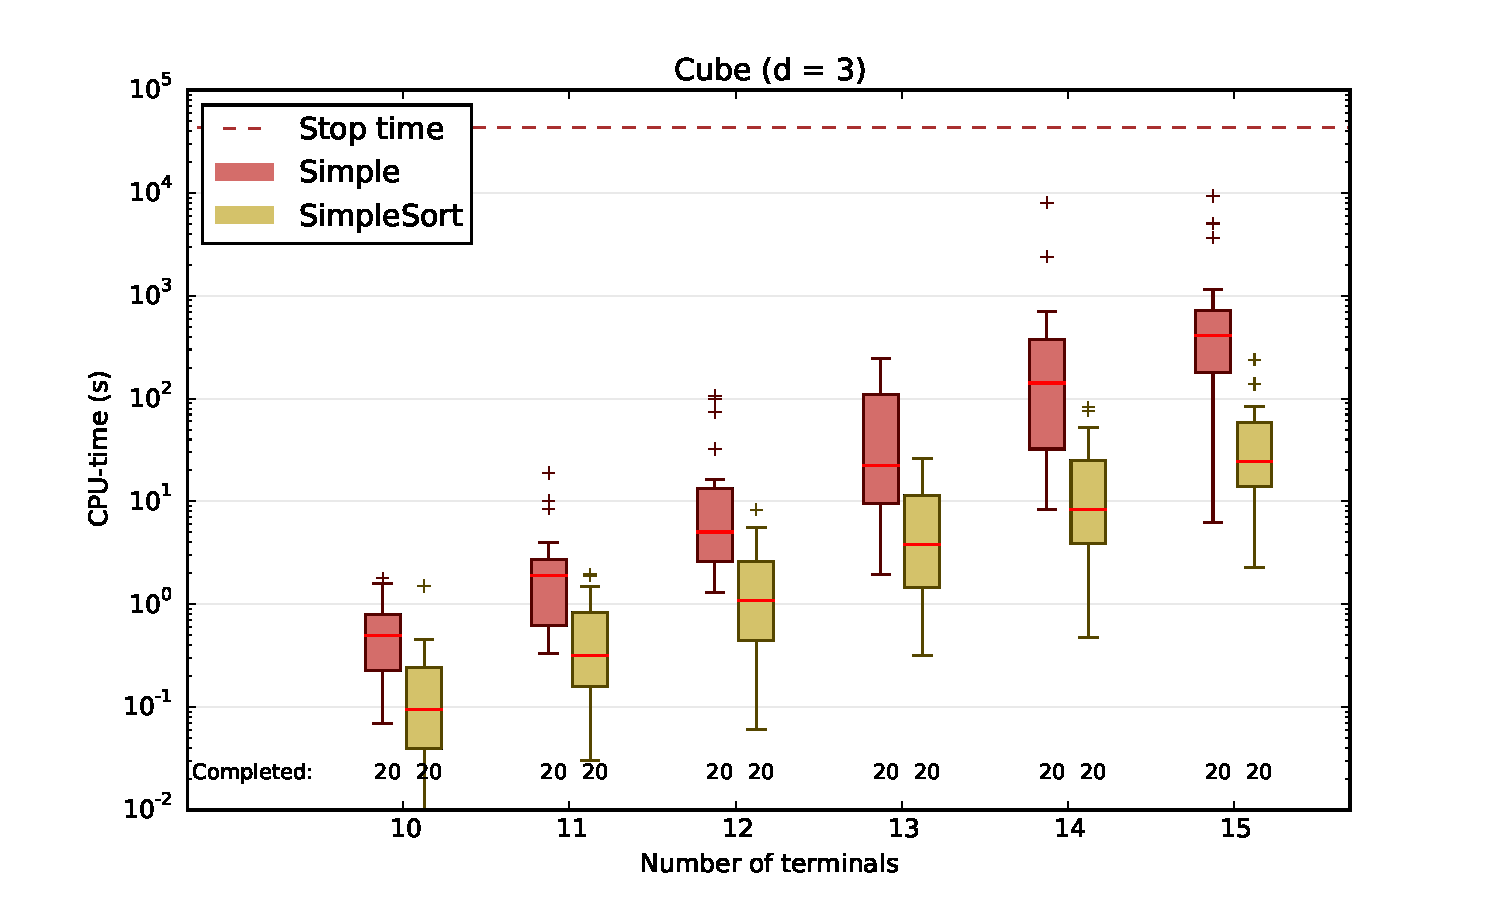
\includegraphics[width=\textwidth]{gfx/boxplots/plot_nvst_boxplot_d3_Cube_3}
  \end{subfigure}%
  \begin{subfigure}[t]{0.5\textwidth}
    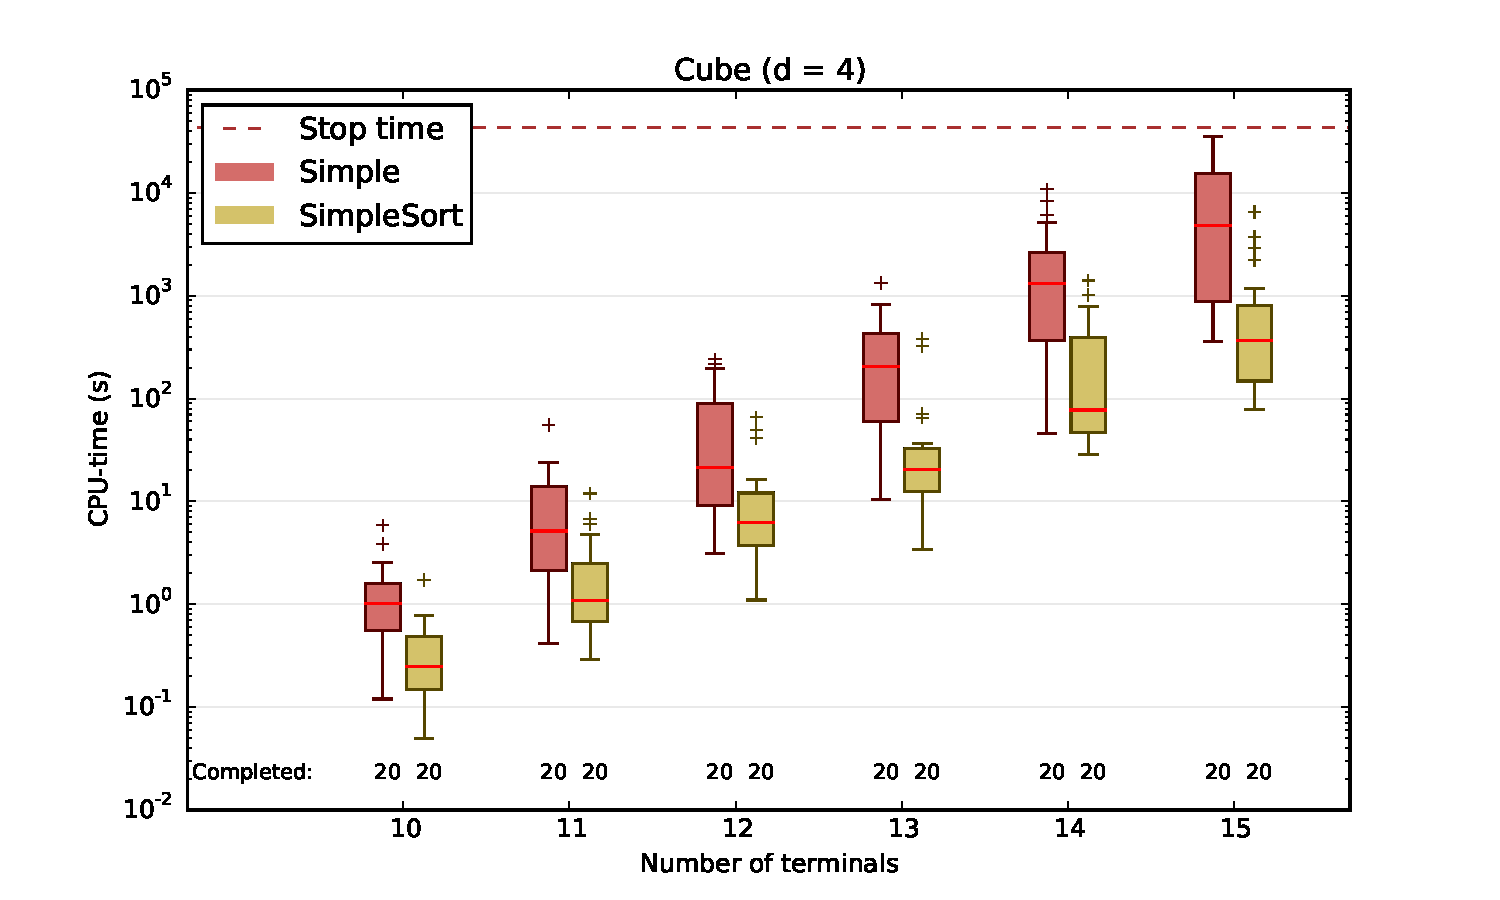
\includegraphics[width=\textwidth]{gfx/boxplots/plot_nvst_boxplot_d4_Cube_3}
  \end{subfigure}%
  \caption[Box-plots: Unsorted terminals vs.\ sorted terminals]{Box-plots for
    the Cube set for $d = 3,4$, plotting the run-times for the sorted and
    unsorted terminals. For a description of the plots legend and appearance see
    the description in~\cref{fig:boxplots-1}.\label{fig:boxplots-2}}
\end{figure}
%
To further compare the effect of sorting the terminals as described
in~\cref{sec:sorting-terminals}, box-plots for the Cube set with $d = 3$ and $d
= 4$ has been plotted for \texttt{SmithNew} vs.\ \texttt{SmithNewSort} and
\texttt{Simple} vs.\ \texttt{SimpleSort}. These can be found
in~\cref{fig:boxplots-2}. As can be seen from the figures, the run-time of both
methods drop significantly when the terminals are sorted. In almost all cases,
no matter the number of terminals, is the third quartile of the sorted terminals
below the first quartile of the unsorted terminals. The proposed way of sorting
the terminals thus seems to work very well. Also notice, that sorting the
terminals improves the new implementations run-time enough that
\texttt{SmithNewSort} has run-times comparable to/slightly better than
\texttt{SmithOld}.

The reason that the dimensions $d=2$ and $d=5$ have not been plotted is, both
that they show the same situation, but also that $d=2$ is so small that they go
below the graph, and would require another a change of y-axis, and $d=5$ has a
bit to few solved instances for $n=15$ for it to be quite as reliable.

\subsection{Trees and Iterations}
\label{sec:trees-iterations}

Apart from the actual run-time of the implementation, another metric worth
measuring is the number of optimization iterations one runs when solving an
instance, and the number of trees optimized. By the last what is the number of
topology vectors on which we optimize their corresponding tree at least once.
%
\begin{table}[htbp]
  \centering
  \scalebox{0.7}{
  \begin{tabular}{ccccccc}
    \toprule
         &     & \multicolumn{5}{c}{Method}                               \\
    \cmidrule(l){3-7}
    $n$  & $d$ & \texttt{Simple} & \texttt{SimpleSort} & \texttt{SmithNew} & \texttt{SmithNewSort} & \texttt{SmithOld} \\
    \cmidrule(r){1-2}\cmidrule(l){3-7}
    $10$ & $2$ & $1.04$ & $0.13$     & $1.42$   & $0.17$       & $1.00$   \\
         & $3$ & $1.21$ & $0.25$     & $1.70$   & $0.37$       & $1.00$   \\
         & $4$ & $1.17$ & $0.60$     & $1.61$   & $0.89$       & $1.00$   \\
         & $5$ & $1.54$ & $0.85$     & $2.25$   & $1.34$       & $1.00$   \\
    \cmidrule(r){1-2}
    $11$ & $2$ & $1.05$ & $0.10$     & $1.62$   & $0.13$       & $1.00$   \\
         & $3$ & $1.23$ & $0.19$     & $1.90$   & $0.29$       & $1.00$   \\
         & $4$ & $1.47$ & $0.36$     & $1.97$   & $0.56$       & $1.00$   \\
         & $5$ & $1.54$ & $0.77$     & $2.57$   & $1.22$       & $1.00$   \\
    \cmidrule(r){1-2}
    $12$ & $2$ & $1.17$ & $0.08$     & $1.90$   & $0.11$       & $1.00$   \\
         & $3$ & $1.42$ & $0.16$     & $2.34$   & $0.25$       & $1.00$   \\
         & $4$ & $1.73$ & $0.26$     & $2.83$   & $0.52$       & $1.00$   \\
         & $5$ & $1.53$ & $0.59$     & $2.24$   & $1.11$       & $1.00$   \\
    \cmidrule(r){1-2}
    $13$ & $2$ & $1.11$ & $0.05$     & $2.22$   & $0.09$       & $1.00$   \\
         & $3$ & $1.43$ & $0.12$     & $2.80$   & $0.20$       & $1.00$   \\
         & $4$ & $0.74$ & $0.25$     & $3.19$   & $0.43$       & $1.00$   \\
         & $5$ & $1.66$ & $0.45$     &          & $1.14$       & $1.00$   \\
    \cmidrule(r){1-2}
    $14$ & $2$ & $0.97$ & $0.05$     & $2.63$   & $0.08$       & $1.00$   \\
         & $3$ & $1.61$ & $0.10$     & $3.44$   & $0.19$       & $1.00$   \\
         & $4$ & $1.52$ & $0.16$     &          & $0.39$       & $1.00$   \\
         & $5$ &        &            &          &              &          \\
    \cmidrule(r){1-2}
    $15$ & $2$ & $1.32$ & $0.04$     & $3.12$   & $0.06$       & $1.00$   \\
         & $3$ &        &            &          &              &          \\
         & $4$ &        &            &          &              &          \\
         & $5$ &        &            &          &              &          \\
    \bottomrule
  \end{tabular}
  }
  \caption[Tree-exploration ratio for Sausage]{The table shows the ratio of
    trees optimized in relation to \texttt{OldSmith}. The number of trees is
    measured such that if a topology vector has been optimized at least once,
    then the number of optimized trees is optimized by one. Topologies that are
    pruned before any optimization has taken place is not counted, and any
    topology can at max be counted once. The data shown are from the Sausage
    set. An empty field means that either the instance for that method, or the
    instance for \texttt{SmithOld} could not be solved within the time limit.\label{tab:trees-sausage-ratio}}
\end{table}
%
\cref{tab:trees-sausage-ratio} shows the number of trees optimized, as a ratio
of the tree optimized by \texttt{SmithOld}, and
\cref{tab:iterations-sausage-ratio} shows the number of iterations, also as a
ratio. Both of these tables are for the Sausage set. As can be seen by the
tables the new implementation, when not sorting terminals, optimizes more trees
than the original implementation. Especially \texttt{SmithNew} in some instances
optimize  
This essentially means it 
%
\begin{table}[htbp]
\centering
  \scalebox{0.7}{
\begin{tabular}{ccccccc}
\toprule
     &     & \multicolumn{5}{c}{Method}                 \\
\cmidrule(l){3-7}
  $n$  & $d$ & \texttt{Simple} & \texttt{SimpleSort} & \texttt{SmithNew} & \texttt{SmithNewSort} & \texttt{SmithOld} \\
\cmidrule(r){1-2}\cmidrule(l){3-7}
$10$ & $2$ & $0.15$ & $0.03$ & $1.10$ & $0.14$ & $1.00$ \\
     & $3$ & $0.23$ & $0.04$ & $1.47$ & $0.28$ & $1.00$ \\
     & $4$ & $0.23$ & $0.08$ & $1.49$ & $0.53$ & $1.00$ \\
     & $5$ & $0.29$ & $0.18$ & $1.37$ & $1.10$ & $1.00$ \\
\cmidrule(r){1-2}
$11$ & $2$ & $0.14$ & $0.02$ & $1.13$ & $0.08$ & $1.00$ \\
     & $3$ & $0.20$ & $0.03$ & $1.57$ & $0.18$ & $1.00$ \\
     & $4$ & $0.24$ & $0.05$ & $1.57$ & $0.32$ & $1.00$ \\
     & $5$ & $0.24$ & $0.08$ & $1.56$ & $0.58$ & $1.00$ \\
\cmidrule(r){1-2}
$12$ & $2$ & $0.14$ & $0.01$ & $1.18$ & $0.06$ & $1.00$ \\
     & $3$ & $0.19$ & $0.02$ & $1.69$ & $0.16$ & $1.00$ \\
     & $4$ & $0.24$ & $0.03$ & $1.67$ & $0.29$ & $1.00$ \\
     & $5$ & $0.22$ & $0.05$ & $1.81$ & $0.40$ & $1.00$ \\
\cmidrule(r){1-2}
$13$ & $2$ & $0.12$ & $0.01$ & $1.23$ & $0.04$ & $1.00$ \\
     & $3$ & $0.17$ & $0.01$ & $1.83$ & $0.12$ & $1.00$ \\
     & $4$ & $0.09$ & $0.03$ & $1.98$ & $0.21$ & $1.00$ \\
     & $5$ & $3.18$ & $0.73$ &        & $8.76$ & $1.00$ \\
\cmidrule(r){1-2}
$14$ & $2$ & $0.09$ & $0.01$ & $1.32$ & $0.03$ & $1.00$ \\
     & $3$ & $0.17$ & $0.01$ & $2.03$ & $0.10$ & $1.00$ \\
     & $4$ & $0.63$ & $0.06$ &        & $0.71$ & $1.00$ \\
     & $5$ &        &        &        &        &        \\
\cmidrule(r){1-2}
$15$ & $2$ & $0.12$ & $0.00$ & $1.42$ & $0.02$ & $1.00$ \\
     & $3$ &        &        &        &        &        \\
     & $4$ &        &        &        &        &        \\
     & $5$ &        &        &        &        &        \\
\bottomrule
\end{tabular}
}
  \caption[Iteration ratio for Sausage]{The table shows the ratio of iterations
     in relation to \texttt{SmithOld} for the Sausage set. The structure is as
     in~\cref{tab:trees-sausage-ratio}. However an iteration means every time we
     perform an optimization, i.e.\ a tree can contribute many times to this if
     we run the iteration for multiple times on the tree (which we most likely
     do).\label{tab:iterations-sausage-ratio}}
\end{table}
%
% \begin{table}[htbp]
%   \centering
%   \scalebox{0.7}{
%   \begin{tabular}{cccccc}
%     \toprule
%          & \multicolumn{5}{c}{Method}                               \\
%     \cmidrule(l){2-6}
%     $n$  & \texttt{Simple} & \texttt{SimpleSort} & \texttt{SmithNew} & \texttt{SmithNewSort} & \texttt{SmithOld} \\
%     \cmidrule(r){1-1}\cmidrule(l){2-6}
%     $4$  & $0.24$ & $0.25$     & $0.99$   & $0.99$       & $1.00$   \\
%     $6$  & $0.34$ & $0.33$     & $0.98$   & $1.01$       & $1.00$   \\
%     $8$  & $0.28$ & $0.26$     & $1.38$   & $1.19$       & $1.00$   \\
%     $12$ & $0.17$ & $0.12$     & $1.49$   & $1.51$       & $1.00$   \\
%     $20$ &        &            &          &              &          \\
%     \bottomrule
%   \end{tabular}
%   }
%   \caption[Iteration ratio for Solids]{The table shows the ratio of iterations
%      in relation to \texttt{SmithOld} for the Solids set. The structure is as
%      in~\cref{tab:trees-sausage-ratio}.\label{tab:iterations-solids-ratio}}
% \end{table}

%%% Local Variables:
%%% mode: latex
%%% TeX-master: "../../main"
%%% End:
